\documentclass{magnolia}

\magtex{tex_driver={pdftex}}
\magfiche{document_nom={Structure séquentielle},
          auteur_nom={François Fayard},
          auteur_mail={francois.fayard@auxlazaristeslasalle.fr}}
\magexos{exos_matiere={maths},
         exos_niveau={mpsi},
         exos_chapitre_numero={4},
         exos_theme={Structure séquentielle}}
\magmisenpage{}
\maglieudiff{}
\magprocess

\begin{document}

%BEGIN_BOOK
\magsection{Liste}
\magsubsection{Liste}
\magsubsection{Parcours de liste}

\exercice{nom={Listes bicolores}}
Soit {\tt L} une liste d'entiers. On dit que {\tt L} est {\it bicolore} si on peut la séparer en deux sous-listes monotones de sens contraires. Par exemple, la liste {\tt [1, 2, 3, 5, 6, 10, 8, 3, 2]} est bicolore car on peut la séparer en {\tt [1, 2, 3, 5, 6] + [10, 8, 3, 2]}. En revanche, la liste {\tt [4, 5, 6, 2, 4]} n'est pas bicolore. Par convention, les listes monotones sont bicolores.\\

Écrire une fonction {\tt bicolore(t: list[int]) -> bool} qui prend en argument une liste
{\tt t} et renvoie le booléen {\tt True} si la liste {\tt t} est bicolore et le booléen {\tt False} sinon.

\exercice{nom={Plus petit entier manquant}}
Écrire une fonction \verb!entier_manquant(t: list[int]) -> int! qui renvoie le plus petit entier naturel absent
d'un tableau d'entiers naturels. Par exemple, pour \verb!t = [1, 3, 7, 6, 4, 1, 2, 0]!, cette fonction devra
renvoyer 5.

\magsubsection{Création de liste}

\exercice{nom={Nombre d'occurences}}
Écrire une fonction \verb!occ(a: list[int], m: int) -> list[int]! prenant en entrée une liste d'entiers
\verb!a! telle que tous ses éléments $k$ vérifient $0\leq k<m$, et renvoyant un tableau $t$ de longueur
$m$ telle que pour tout $k\in\interefo{0}{m}$, \verb!t[k]! est le nombre d'occurences de $k$ dans la
liste \verb!a!.

\magsubsection{Modification des éléments}


\exercice{nom={Rotation}}
On appelle rotation d'un tableau $t$ le fait de décaler tous les éléments d'une place vers
la droite, à l'exception du dernier qui est placé en première place. Par exemple, la rotation
du tableau \verb![1, 2, 3, 4]! est le tableau \verb![4, 1, 2, 3]!.
\begin{questions}
\question Rédiger une fonction \verb!rotation(t: list[int]) -> list[int]! qui renvoie un nouveau tableau égal à la
  rotation du tableau initial.
\question Rédiger une fonction \verb!rotation_en_place(t: list[int]) -> NoneType! qui modifie le tableau pour le
  remplacer par sa rotation.
\question Rédiger une fonction \verb!rotation_multiple(t: list[int], k: int) -> list[int]! qui renvoie un nouveau tableau
  égal à $k$ rotations du tableau $t$.
\end{questions}

% \exercice{nom={Le tri à bulle}}
\exercice{nom={Partition, drapeaux hollandais}}
On suppose que l'on dispose d'une fonction \verb!swap(t: list[int], i: int, j: int) -> NoneType!
qui échange les éléments d'indice $i$ et $j$ dans le tableau $t$.
\begin{questions}
\question On souhaite écrire une fonction \verb!partition(t: list[int], p: int) -> NoneType!
  qui prend en entrée un tableau de longueur $n$ et qui le réordonne afin que tous les éléments
  du tableau strictement inférieurs à $p$ se retrouvent en début de tableau et que tous ceux
  qui sont supérieurs ou  égaux à $p$ se retrouvent en fin de tableau. On effectuera au plus
  $n$ appels à \verb!swap!.  Par exemple, avec $p=6$, le tableau
\begin{center}
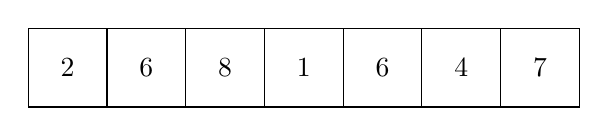
\begin{tikzpicture}
\filldraw [fill=white, draw=black] (0,0) rectangle (1,1) node[pos=.5] {2};
\filldraw [fill=white, draw=black] (1,0) rectangle (2,1) node[pos=.5] {6};
\filldraw [fill=white, draw=black] (2,0) rectangle (3,1) node[pos=.5] {8};
\filldraw [fill=white, draw=black] (3,0) rectangle (4,1) node[pos=.5] {1};
\filldraw [fill=white, draw=black] (4,0) rectangle (5,1) node[pos=.5] {6};
\filldraw [fill=white, draw=black] (5,0) rectangle (6,1) node[pos=.5] {4};
\filldraw [fill=white, draw=black] (6,0) rectangle (7,1) node[pos=.5] {7};
\end{tikzpicture}
\end{center}
sera par exemple transformé en
\begin{center}
\begin{tikzpicture}
\filldraw [fill=colorLazoBlue1Light, draw=black] (0,0) rectangle (1,1) node[pos=.5] {2};
\filldraw [fill=colorLazoBlue1Light, draw=black] (1,0) rectangle (2,1) node[pos=.5] {1};
\filldraw [fill=colorLazoBlue1Light, draw=black] (2,0) rectangle (3,1) node[pos=.5] {4};
\filldraw [fill=colorLazoPink1Light, draw=black] (3,0) rectangle (4,1) node[pos=.5] {6};
\filldraw [fill=colorLazoPink1Light, draw=black] (4,0) rectangle (5,1) node[pos=.5] {6};
\filldraw [fill=colorLazoPink1Light, draw=black] (5,0) rectangle (6,1) node[pos=.5] {8};
\filldraw [fill=colorLazoPink1Light, draw=black] (6,0) rectangle (7,1) node[pos=.5] {7};
\end{tikzpicture}
\end{center}
On pourra pour cela initialiser des variables $i$ et $j$ à 0 et
maintenir l'invariant suivant
\begin{center}
\begin{tikzpicture}
\filldraw [fill=colorLazoBlue1Light, draw=black] (0,0) rectangle (1,1) node[pos=.5] {2};
\filldraw [fill=colorLazoBlue1Light, draw=black] (1,0) rectangle (2,1) node[pos=.5] {1};
\filldraw [fill=colorLazoPink1Light, draw=black] (2,0) rectangle (3,1) node[pos=.5] {8};
\filldraw [fill=colorLazoPink1Light, draw=black] (3,0) rectangle (4,1) node[pos=.5] {6};
\filldraw [fill=white, draw=black] (4,0) rectangle (5,1) node[pos=.5] {6};
\filldraw [fill=white, draw=black] (5,0) rectangle (6,1) node[pos=.5] {4};
\filldraw [fill=white, draw=black] (6,0) rectangle (7,1) node[pos=.5] {7};
\node[] at (0.5,-0.25) {0};
\node[] at (1.5,-0.25) {1};
\node[] (B) at (2.5,-0.25) {2};
\node[] at (3.5,-0.25) {3};
\node[] (D) at (4.5,-0.25) {4};
\node[] at (5.5,-0.25) {5};
\node[] at (6.5,-0.25) {6};
\node[] (A) at (2.5,-1.25) {$i$};
\node[] (C) at (4.5,-1.25) {$j$};
\draw[->] (A)--(B);
\draw[->] (C)--(D);
\end{tikzpicture}
\end{center}
La variable $i$ indiquant la fin de la zone bleue des entiers $< p$ déjà traités et
la variable $j$ indiquant la fin de la zone rose des entiers $\geq p$ déjà traités,
l'indice $j$ étant l'indice du prochain entier à traiter.
\question Écrire une fonction \verb!partition_hollandais(t: list[int], p: int) -> NoneType! qui prend
  en entrée une liste $t$ de longueur $n$ et qui le réordonne en 3 zones successives~:
  les entiers strictement inférieurs à $p$, les entiers égaux à $p$ et ceux strictement
  supérieurs à $p$. On effectuera au plus $2n$ appels à \verb!swap!.
\question Modifier la fonction précédente afin qu'elle n'effectue qu'au plus $n$ appels
  à \verb!swap!.
\end{questions}



\magsubsection{Ajout et suppression d'éléments}

\exercice{nom={Fusion}}
Écrire une fonction \verb!fusion(t1: list[int], t2: list[int]) -> list[int]! qui prend en
entrée deux listes triées dans l'ordre croissant et qui renvoie une liste triée dans
l'ordre croissant contenant les entiers des deux listes. On pourra compléter le programme
suivant~:
\begin{pythoncode}
def fusion(t1, t2):
    """fusion(t1: list[int], t2: list[int]) -> list[int]"""
    i1 = 0
    i2 = 0
    t = []
    while i1 < len(t1) and i2 < len(t2):
        ...
    ...
\end{pythoncode}


\magsubsection{Les objets Python}
\magsection{Structures séquentielles}
\magsubsection{Pile}


\exercice{nom={Calculatrice polonaise inverse}}
L'écriture polonaise inverse des expressions arithmétiques place l'opérateur après les
opérandes. Cette notation ne nécessite aucune parenthèse ni aucune règle de priorité.
Ainsi, l'expression polonaise inverse décrite par la liste
\verb![1, 2, 3, '*', '+', 4, '*']! désigne l'expression traditionnellement notée $(1+2\times 3)\times 4$.
La valeur d'une telle expression peut être calculée facilement en utilisant une pile pour
stocker les résultats intermédiaires. Pour cela, on observe un à un les éléments de
l'expression et on effectue les actions suivantes~:
\begin{itemize}
\item Si on voit un nombre, on le place sur la pile.
\item Si on voit un opérateur binaire, on récupère les deux nombres au sommet de la pile,
  on leur applique l'opérateur, et à la fin du processus il reste exactement un nombre sur
	la pile qui est le résultat.
\end{itemize}
Écrire une fonction \verb!eval(a: list) -> int! prenant en paramètre une liste représentant une expression
en notation polonaise inverse composée d'additions et de multiplications de nombres entiers
et renvoyant la valeur de cette expression. Par exemple \verb!eval([1, 2, 3, '*', '+', 4, '*'])!
devra renvoyer 28.


\magsubsection{File}


\exercice{nom={Temps d'attente}}
Dans cet exercice, on se propose d'évaluer le temps d'attente de clients à des guichets, en
comparant la solution d'une unique file d'attente et la solution d'une file d'attente par
guichet. Pour cela, on modélise le temps par une variable globale, qui est incrémentée
à chaque tour de boucle. Lorsqu'un nouveau client arrive, il est placé dans une file
sous la forme d'un entier égal à la valeur de l'horloge, c'est-à-dire égal à son heure
d'arrivée. Lorsqu'un client est servi, c'est-à-dire lorsqu'il sort de sa file d'attente, on
obtient son temps d'attente en faisant la soustraction de la valeur courante de l'horloge
et de la valeur qui vient d'être retirée de la file. L'idée est de faire tourner une telle
simulation relativement longtemps, tout en totalisant le nombre le nombre de clients servis
et le temps d'attente cumulé sur tous les clients. Le rapport de ces deux quantités nous
donne le temps d'attente moyen. On peut alors comparer plusieurs stratégies (une ou plusieurs
files, choix d'une file au hasard lorsqu'il y en a plusieurs, choix de la file où il y a le
moins de clients, etc).\\
On se donne un nombre $n$ de guichets (par exemple $n=5$). Pour simuler la disponibilité d'un
guichet, on peut se donner un tableau d'entiers \verb!dispo! de taille $n$. La valeur de
\verb!dispo[i]! indique le nombre de tours d'horloge où le guichet $i$ sera occupé. En
particulier, lorsque cette valeur vaut 0, cela veut dire que le guichet est libre et peut donc
servir un nouveau client. Lorsqu'un client est servi par le guichet $i$, on choisit un temps
de traitement pour ce client, au hasard entre 0 et $n$ et on l'affecte à \verb!dispo[i]!. À
chaque tour d'horloge, on réalise deux opérations~:
\begin{itemize}
\item On fait apparaitre un nouveau client.
\item Pour chaque guichet $i$
  \begin{itemize}
	\item S'il est disponible, il sert un nouveau client (pris dans sa propre file ou dans
	  l'unique file, selon le modèle), le cas échéant.
	\item sinon, on décrémente \verb!dispo[i]!.
	\end{itemize}
\end{itemize}
Écrire un programme qui effectue une telle simulation, sur $100\ 000$ tours d'horloge, et
affiche au final le temps d'attente moyen. Comparer avec différentes stratégies.

\magsubsection{File de priorité}
\magsubsection{Dictionnaire}

\exercice{nom={Somme donnée}}

On cherche à écrire une fonction prenant en entrée une liste d'entiers \verb!t! et un entier \verb!s! et
qui nous indique si la liste possède deux entiers dont la somme vaut \verb!s!.
\begin{questions}
\question Écrire une telle fonction \verb!somme(t: list[int], s: int) -> bool! répondant à la question.
\question On souhaite désormais écrire une version plus efficace de cette fonction qui ne parcourt qu'une
  seule fois la liste. En maintenant à jour l'ensemble des entiers déjà observés, écrire une fonction
  répondant à la même question et ne parcourant qu'une seule fois la liste.
\end{questions}


% \exercice{nom={Écriture des chiffres d'un entier en base 2}}
% Écrire une fonction \textsc{Python} {\tt Vers\_base2(n)} dont l'appel renvoie la liste des chiffres de l'écriture de l'entier $n$ en base 2 en commençant par les chiffres de poids forts.

% \exercice{nom={Le crible d'Ératosthène}}
% \begin{enumerate}
% \item Écrire une fonction \textsc{Python} {\tt barre(l,j)} qui prend en argument une liste d'entiers naturels {\tt l} et un entier naturel non nul {\tt j}, qui remplace par 0 le contenu de toutes les cases de {\tt l} d'index $> j$ et divisible par $j$. Cette fonction agira par effet de bord et ne renverra rien.
% \item En s'appuyant sur la méthode du crible d'Ératosthène, écrire une fonction \textsc{Python} {\tt Premiers(n)} qui prend en argument un entier naturel $n$ non nul, et dont l'appel renvoie la liste de tous les nombres premiers inférieurs ou égaux à $n$.
% \end{enumerate}



% \exercice{nom={Recherche d'un élément dans une liste : le cas général}}
% Écrire une fonction \textsc{Python} {\tt ixina(x,A)} prenant en argument un entier {\tt x} et une liste d'entiers {\tt A} et dont l'appel renvoie le booléen {\tt True} si {\tt x} est présent dans la liste {\tt A} et {\tt False} sinon. Essayer de trouver une solution ne nécessitant pas de parcourir toute la liste si {\tt x} est présent dans {\tt A}.

% \exercice{nom={Le cas d'une liste triée : la recherche dichotomique}}
% Pour chercher $x$ dans la liste triée par ordre croissant $[a_0,\dots,a_{n-1}]$, on applique la méthode de {\it dichotomie} : on compare $x$ et $a_p$ avec $p=\lfloor \frac{n-1}{2} \rfloor$ (pourquoi cette valeur de $p$ ? parce que $0 + n-1 = n-1$, vous verrez) :
% \begin{itemize}
% \item si $x<a_p$, alors x, s'il se trouve dans la liste, ne peut qu'être dans la liste $[a_0,\dots,a_{p-1}]$ ;
% \item si $x>a_p$, alors x, s'il se trouve dans la liste, ne peut qu'être dans la liste $[a_{p+1},\dots,a_{n-1}]$ ;
% \item si $x=a_p$, alors la recherche est terminée.
% \end{itemize}
% La mise en \oe{}uvre pratique utilise deux variables entières $g$ et $d$ délimitant le domaine $[a_g,\dots,a_d]$ dans lequel on cherche $x$. Les valeurs initiales de ces variables sont donc $g=0$ et $d=n-1$. On compare ensuite $x$ à l'élément médian d'index  $m=\lfloor \frac{g+d}{2} \rfloor$, et, si nécessaire, on poursuit la recherche en remplaçant $d$ par $m-1$ ou $g$ par $m+1$. La recherche s'achève (par une réponse négative) lorsque $d<g$ puisqu'alors le domaine de recherche est vide.
% \begin{enumerate}
% 	\item Écrire une fonction \textsc{Python} {\tt dichot(x,l)} qui prend en argument un entier {\tt x} et une liste d'entiers {\tt l} triée par ordre croissant, et qui renvoie {\tt True} ou {\tt False} selon que {\tt x} est présent dans la liste {\tt l} ou non, et qui utilise la méthode de dichotomie telle qu'exposée ci-dessus.
% 	\item Il y a bien d'autres façons de programmer la méthode de dichotomie.  Voici deux tentatives, très ressemblantes. Ces fonctions répondent-elles à la question ? 
% \begin{pythoncode}
% def dichot_v2(x,l):                  def dichot_v3(x,l): 
% 		g = 0                                g = 0
% 		d = len(l)-1                         d = len(A) - 1 
% 		while g < d:                         while g < d:
% 				m = (g+d)//2                         m = (g+d) // 2
% 				if x > l[m]:                         if x < l[m]:
% 						g = m+1                              d = m - 1 
% 				else:                                else:
% 						d = m                                g = m
% 		return l[g] == x                     return l[g] == x  
% \end{pythoncode}

% {\it Indications} : Pour la preuve de validité, on pourra considérer la propriété ($\mathcal{H}$) suivante: "L'élément {\tt x} est présent dans la liste {\tt l} si et seulement si il est présent dans la sous-liste {\tt [l[i] for i in range(g,d)]}" et montrer que c'est un invariant de boucle. Pour la preuve de terminaison, on pourra considérer la quantité $d-g$. Si ça ne marche pas, on pourra tester les fonctions sur des listes de longueur 1 ou 2.
% \end{enumerate}

% \exercice{nom={Les polynômes en Python}}
% On choisit dans cet exercice de représenter un polynôme par la liste de ses coefficients. Ainsi, le polynôme 
% $P(X)=\sum_{k=0}^n a_k X^k$ sera représenté par la liste $[a_0,\dots,a_n]$. 
% Un même polynôme admet donc plusieurs  représentations distinctes puisque que l'on n'impose pas de condition sur $a_n$. 
% Par exemple, les listes $[1,2,4,5,6,0,0,0,0]$ et $[1,2,4,5,6,0]$ représentent toutes les deux le polynôme $1+2X+4X^2+5X^3+6X^4$.
% \begin{enumerate}
% \item Créer deux listes {\tt a} et {\tt b} représentant les polynômes $A(X)=1+2X-4X^{3}+X^{4}$ et $B(X)=1+X$. 
% \item Écrire une fonction {\tt degre(p: list[int]) -> int} prenant en argument une liste {\tt p} et dont l'appel renvoie le degré du polynôme $P$ représenté par la liste {\tt p}.
% \item Écrire une fonction {\tt sub(p: list[int], q: list[int]) -> list[int]} qui prend en argument deux listes {\tt p} et {\tt q} représentant les polynômes $P$ et $Q$ et dont l'appel renvoie une liste représentant le polynôme $P-Q$.
% \item Écrire une fonction {\tt mult(p: list[int], q: list[int]) -> list[int]} qui prend en argument deux listes {\tt p} et {\tt q} représentant les polynômes $P$ et $Q$ et dont l'appel renvoie une liste représentant le polynôme $P\times Q$.
% \item On considère la suite de polynômes $(T_n)$ définie par
% \[T_0=1,\quad T_1=X,\quad \et\quad \forall n\in\N\qsep T_{n+2}=2 X T_{n+1}-T_n.\]
% Écrire une fonction {\tt tcheby(n: int) -> list[int]} prenant en argument un entier {\tt n} et dont l'appel renvoie une liste représentant le polynôme $T_n$.
% \end{enumerate}





% On suppose que {\tt t} est une liste d'entiers naturels. On note $n$ la longueur de {\tt t}. On cherche à trier cette liste. Pourquoi ? Quitte à anticiper sur le chapitre suivant, disons que le fait d'avoir une liste triée permet d'utiliser ensuite des algorithmes beaucoup plus rapides. Nous verrons par exemple qu'il est beaucoup plus économique de chercher un élément dans une liste si celle-ci est triée.
% Il est donc fondamental de savoir trier efficacement une liste.


% Nous présenterons cette année différents algorithmes plus ou moins efficaces. Ceux que nous allons étudier maintenant sont de type {\it itératif}, nous verrons ultérieurement des algorithmes de tri {\it récursifs}, qui sont plus efficaces (en un sens à préciser).

% Précisons quelques points de terminologie :
% \begin{itemize}
%   \item on dit qu'un algorithme trie {\it en place} une liste si il agit uniquement par permutation des cases de la liste, ce sans créer de liste auxiliaire ; l'avantage d'un tel tri est qu'il est économique en mémoire et est bien adapté pour les objets de type {\tt array} (relax, on verra ça plus tard)
%   \item on dit qu'un algorithme de tri est {\it stable} si l'ordre des éléments égaux est préservé.
% \end{itemize}

% La page Wikipedia consacrée aux algorithmes de tri offre une présentation intéressante du sujet, avec plus d'une vingtaine d'algorithmes présentés et comparés.

% \exercice{nom={Tri par insertion}}
% Le tri par insertion est un des algorithmes les plus simples. C'est celui que vous utilisez pour triez vos cartes lorsque vous jouez au tarot. L'idée est d'insérer, carte après carte, la $i$-ème carte dans le groupe de cartes de gauche qui est déjà trié.

% \medskip
% {\bf Algorithme} :
% \begin{itemize}
%   \item On considère le deuxième élément de $L$, s'il est plus petit que $L[0]$ alors on échange les deux premières cases.
%   \item À l'étape numéro $i$ : on a  déjà trié par ordre croissant les $i$ premières cases de $L$,  on lit $x$ le  $i+1$ ème élément de la liste et par échanges de proche en proche on fait descendre  l'élément  $x$ jusqu'à ce que la liste des $i+1$ premiers éléments soit triée par ordre croissant.
% \end{itemize}
% \begin{enumerate}
% \item Tester à la main l'algorithme sur la liste $[6,1,4,2,2,8]$.
% \item Écrire  une fonction \textsc{Python} {\tt tri\_insert(L)}  qui trie en place la liste $L$ en utilisant l'algorithme de  tri par insertion. 
% Cette fonction agira par effet de bord et ne renverra rien.
% \item Combien cette fonction utilise-t-elle d'échanges entre cases de $L$ au minimum ? au maximum ?
% \item Combien cette fonction utilise-t-elle de comparaisons entre éléments du tableau au minimum ? au maximum ?
% \item Cet algorithme est-il stable ?
% \end{enumerate}

% \exercice{nom={Le tri par sélection}}

% {\bf Algorithme} : On crée une liste {\tt A} qui contient la liste courante des éléments à trier, et une liste {\tt res} qui contient, classés dans l'ordre croissant, les plus petits éléments de {\tt L}.
% \begin{itemize}
%   \item Initialisation : {\tt A = L} et {\tt res = [ ]} 
%   \item Itération : on cherche le minimum de {\tt A}, on l'enlève de {\tt A} et on le rajoute à la fin de la liste {\tt res}.
% \end{itemize}

% \begin{enumerate}
% \item Tester à la main l'algorithme sur la liste $[6,1,4,2,2,8]$.
% \item Écrire une fonction \textsc{Python} {\tt mini(T)} qui prend en argument une liste d'entiers {\tt T} et renvoie un couple {\tt (i,x)} où {\tt x} contient la valeur minimale parmi toutes les cases de {\tt T} et {\tt i} est l'index d'une case de {\tt T} qui contient cette valeur minimale.
% \item Écrire une fonction \textsc{Python} {\tt tri\_select(L)} qui renvoie une liste triée  par ordre croissant et contenant les mêmes éléments que la liste {\tt L}. 
% \item Combien cette fonction utilise-t-elle de comparaisons entre éléments de la liste {\tt L} au minimum ? au maximum ?
% \item Montrer que le tri par sélection est stable.
% \item Écrire une fonction \textsc{Python} {\tt tri\_select\_enplace(L)} dont l'appel trie en place la liste {\tt L} en suivant l'algorithme du tri par sélection. Cette fonction agira par effet de bord et ne renverra rien.
% \item Combien cette fonction utilise-t-elle d'échanges entre cases de {\tt L} au minimum ? au maximum ? 
% \item Montrer que la version en place du tri par sélection n'est pas stable. On pourra considérer la liste {\tt [4a, 4b, 2, 6, 5]}.
% \end{enumerate}

% \exercice{nom={Le tri à bulle}}

% {\bf Algorithme} : On parcourt plusieurs fois la liste. À chaque parcours de la liste, on échange {\tt L[i]} et {\tt L[i+1]} si ces quantités ne sont pas dans l'ordre croissant (ceci a pour effet de faire remonter les plus grands éléments à la fin, comme les bulles de gaz remontent à la surface lorsqu'on secoue un verre de Champagne...). On s'arrête dès qu'aucun échange n'a été effectué au cours de ce parcours.

% \medskip

% \begin{enumerate}
% \item Tester à la main l'algorithme sur la liste $[6,8,4,2,2,3]$. 
% \item Expliquer pourquoi seul le premier parcours doit nécessairement parcourir la totalité de la liste.
% \item Écrire une fonction \textsc{Python} {\tt meilleur\_alafin(L,k,n)} qui fait parcourir à l'indice {\tt i} toutes les valeurs de $0$ à $n-2-k$, et, pour chaque valeur de {\tt i},  échange {\tt L[i]} et {\tt L[i+1]} si {\tt L[i] > L[i+1]} et renvoie un booléen de valeur {\tt True} si et seulement si au moins un échange de cases a été effectué. 
% \item Écrire alors une fonction {\tt tri\_bulle(L)} qui, en exploitant l'algorithme de tri à bulle, trie en place la liste {\tt L}. Cette fonction agira par effet de bord et ne renverra rien.
% \item Combien cette fonction utilise-t-elle de comparaisons entre éléments de la liste {\tt L} ? d'échanges ? au minimum ? au maximum ?
% \item Cet algorithme est-il stable ?
% \end{enumerate}

% \exercice{nom={Le tri par tableau des occurrences}}

% {\bf Algorithme} :
% \begin{itemize}
% \item on parcourt la liste {\tt L} une première fois pour rechercher le maximum $m$ des éléments de 
% cette liste.
% \item on parcourt la liste {\tt L} une deuxième fois pour construire le {\it tableau des occurrences} de {\tt L}.
% Il s'agit d'un tableau de longueur $m+1$ dont la case d'indice $i$ contient le nombre d'occurrences de
% la valeur $i$ dans la liste {\tt L}, c'est-à-dire le nombre de cases de {\tt L} dont le contenu est égal à $i$.
% \item en utilisant le tableau des occurrences, on construit une nouvelle liste, de même longueur que 
% {\tt L}, contenant les mêmes éléments que {\tt L} rangés par ordre croissant.
% \end{itemize}

% \begin{enumerate}
% \item Tester à la main l'algorithme sur la liste $[6,1,4,2,2,6,8,3,6,6]$.
% \item Écrire une fonction {\tt occ(L)} qui renvoie le tableau des occurrences de la liste {\tt L}.
% \item Écrire une fonction {\tt tri-occ(L)} qui trie une liste d'entiers naturels {\tt L} par cette méthode.
% \item Combien cette dernière fonction utilise-t-elle de comparaisons entre éléments de la liste {\tt L} ?
% de lectures de case de la liste {\tt L} ? On exprimera le résultat en fonction de la longueur $n$
% et du maximum $m$ de la liste {\tt L}.
% \item Pour quelles listes cet algorithme de tri par tableau des occurrences est-il particulièrement efficace ?
% Proposer un exemple concret.
% \end{enumerate}


% \magsection{Pile, file}



% \exercice{nom={Parenthèse associée}}
% On dit qu'une chaîne de caractères comprenant, entre autres choses, des parenthèse
% \verb!(! et \verb!)! est bien parenthésée lorsque chaque parenthèse ouvrante est
% associée à une unique parenthèse fermante et réciproquement.\\

% À l'aide d'une pile, écrire une fonction prenant en paramètre une chaîne bien parenthésée
% $s$ et l'indice $j$ d'une parenthèse fermante et qui renvoie l'indice $i$ de la parenthèse
% ouvrante associée.
 



% \exercice{nom={Calculatrice}}
% On souhaite réaliser un programme évaluant une expression arithmétique donnée par une chaîne
% de caractères. On utilisera les notations et les règles de priorité ordinaires, en supposant
% pour simplifier que chaque élément est séparé par les autres par une espace. Ainsi,
% l'expression $(1+2\times 3)\times 4$ sera décrite par la chaîne de caractères
% \verb!'(1 + 2 * 3 ) * 4'!

% J'aurai géré ça avec une pile :
% si le caractère est '(', j'empile son indice dans la chaîne
% si le caractère est ')', 2 cas se présentent :
% soit la pile est vide : c'est une ')' en trop : on stoppe et on retourne son indice
% soit la pile n'est pas vide, on dépile
% une fois la chaîne lue en entier, si la pile est vide, on a une chaîne équilibrée, 
% si elle n'est pas vide, on a la liste de tous les indices avec une '(' en trop.

%END_BOOK

\end{document}
